\documentclass{article}\usepackage{graphicx, color}
%% maxwidth is the original width if it is less than linewidth
%% otherwise use linewidth (to make sure the graphics do not exceed the margin)
\makeatletter
\def\maxwidth{ %
  \ifdim\Gin@nat@width>\linewidth
    \linewidth
  \else
    \Gin@nat@width
  \fi
}
\makeatother

\definecolor{fgcolor}{rgb}{0.2, 0.2, 0.2}
\newcommand{\hlnumber}[1]{\textcolor[rgb]{0,0,0}{#1}}%
\newcommand{\hlfunctioncall}[1]{\textcolor[rgb]{0.501960784313725,0,0.329411764705882}{\textbf{#1}}}%
\newcommand{\hlstring}[1]{\textcolor[rgb]{0.6,0.6,1}{#1}}%
\newcommand{\hlkeyword}[1]{\textcolor[rgb]{0,0,0}{\textbf{#1}}}%
\newcommand{\hlargument}[1]{\textcolor[rgb]{0.690196078431373,0.250980392156863,0.0196078431372549}{#1}}%
\newcommand{\hlcomment}[1]{\textcolor[rgb]{0.180392156862745,0.6,0.341176470588235}{#1}}%
\newcommand{\hlroxygencomment}[1]{\textcolor[rgb]{0.43921568627451,0.47843137254902,0.701960784313725}{#1}}%
\newcommand{\hlformalargs}[1]{\textcolor[rgb]{0.690196078431373,0.250980392156863,0.0196078431372549}{#1}}%
\newcommand{\hleqformalargs}[1]{\textcolor[rgb]{0.690196078431373,0.250980392156863,0.0196078431372549}{#1}}%
\newcommand{\hlassignement}[1]{\textcolor[rgb]{0,0,0}{\textbf{#1}}}%
\newcommand{\hlpackage}[1]{\textcolor[rgb]{0.588235294117647,0.709803921568627,0.145098039215686}{#1}}%
\newcommand{\hlslot}[1]{\textit{#1}}%
\newcommand{\hlsymbol}[1]{\textcolor[rgb]{0,0,0}{#1}}%
\newcommand{\hlprompt}[1]{\textcolor[rgb]{0.2,0.2,0.2}{#1}}%

\usepackage{framed}
\makeatletter
\newenvironment{kframe}{%
 \def\at@end@of@kframe{}%
 \ifinner\ifhmode%
  \def\at@end@of@kframe{\end{minipage}}%
  \begin{minipage}{\columnwidth}%
 \fi\fi%
 \def\FrameCommand##1{\hskip\@totalleftmargin \hskip-\fboxsep
 \colorbox{shadecolor}{##1}\hskip-\fboxsep
     % There is no \\@totalrightmargin, so:
     \hskip-\linewidth \hskip-\@totalleftmargin \hskip\columnwidth}%
 \MakeFramed {\advance\hsize-\width
   \@totalleftmargin\z@ \linewidth\hsize
   \@setminipage}}%
 {\par\unskip\endMakeFramed%
 \at@end@of@kframe}
\makeatother

\definecolor{shadecolor}{rgb}{.97, .97, .97}
\definecolor{messagecolor}{rgb}{0, 0, 0}
\definecolor{warningcolor}{rgb}{1, 0, 1}
\definecolor{errorcolor}{rgb}{1, 0, 0}
\newenvironment{knitrout}{}{} % an empty environment to be redefined in TeX

\usepackage{alltt}
\usepackage{amsmath}
\usepackage{natbib}
\title{Cointegration}
\author{Rob Hayward}
\IfFileExists{upquote.sty}{\usepackage{upquote}}{}
\begin{document}
\maketitle
\section{Introduction}
This paper will examine time series with a focus on stationarity, integration and cointegration. The first part discusses tests for stationarity, the second looks at cointegration and the methods used to identify cointegrated series. 

\section{Stationary data}
A standard series to be investigated can take the form of 
\begin{equation}
y_t = TD_t + z_t
\end{equation}

Where $y_t$ is the series of attention, $TD_t$ is the deterministic component that takes the form of $TD_t = \beta_0 + \beta_1 t$ and $z_t$ is the stochastic part that is assumed to be an autoregressive-moving average process of the form $\Phi L(z_t) = \theta L(z_t) \varepsilon_t$,  with $\varepsilon_t \sim iid$. 

It is possible to differentiate between \emph{trend stationary} 

\begin{equation}
y_t = y_{t-1} + \mu = y_0 + \mu t
\end{equation}

and \emph{difference stationary} processes.  

\begin{equation}
y_t = y_{t-1} + \varepsilon = y_0 + \sum_{i=0}^t \varepsilon_t
\end{equation}

If all the roots of the autoregressive polynominal $\phi_p(z)$ lie outside the unit circle, the process is stationary (possibly trend stationary); if at least one of the roots lies on the unit circle and there is a unit root and then the process is difference statonary. 

\begin{equation}
\phi_p(z) = 1 - \phi_1 (z) - \phi_2(z)^2 - \phi_3(z)^3...\phi_p(z)^p
\end{equation}
 
It is possible to create and plot these different types of time series.  
\begin{knitrout}
\definecolor{shadecolor}{rgb}{0.969, 0.969, 0.969}\color{fgcolor}\begin{kframe}
\begin{alltt}
\hlfunctioncall{set.seed}(123456)
e <- \hlfunctioncall{rnorm}(500)
rw.nd <- \hlfunctioncall{cumsum}(e)
\end{alltt}
\end{kframe}
\end{knitrout}

After setting the seed and generating 500 norman random variables $(e)$. 
\begin{knitrout}
\definecolor{shadecolor}{rgb}{0.969, 0.969, 0.969}\color{fgcolor}\begin{kframe}
\begin{alltt}
trd <- 1:500
\end{alltt}
\end{kframe}
\end{knitrout}

The \emph{random walk} $(rw.nd)$ is the cumulation $(cumsum(e))$ of the normal random variable.
\begin{knitrout}
\definecolor{shadecolor}{rgb}{0.969, 0.969, 0.969}\color{fgcolor}\begin{kframe}
\begin{alltt}
rw.wd <- 0.5 * trd + \hlfunctioncall{cumsum}(e)
\end{alltt}
\end{kframe}
\end{knitrout}

By creating a trend $(trd)$ a \emph{random walk with drift} can be established with a combination of the cumulative shock and a constant drift $(rw.wd)$.
\begin{knitrout}
\definecolor{shadecolor}{rgb}{0.969, 0.969, 0.969}\color{fgcolor}\begin{kframe}
\begin{alltt}
dt <- e + 0.5 * trd
\end{alltt}
\end{kframe}
\end{knitrout}

A \emph{deterministic trend with noise} $(dt)$ combines the tend $(trd)$ with noise $(e)$.

Now plot the three series. 
\begin{knitrout}
\definecolor{shadecolor}{rgb}{0.969, 0.969, 0.969}\color{fgcolor}\begin{kframe}
\begin{alltt}
\hlfunctioncall{par}(mar = \hlfunctioncall{rep}(5, 4))
\hlfunctioncall{plot.ts}(dt, lty = 1, ylab = \hlstring{""}, xlab = \hlstring{""})
\hlfunctioncall{lines}(rw.wd, lty = 2)
\hlfunctioncall{par}(new = T)
\hlfunctioncall{plot.ts}(rw.nd, lty = 3, axes = FALSE)
\hlfunctioncall{axis}(4, \hlfunctioncall{pretty}(\hlfunctioncall{range}(rw.nd)))
\hlfunctioncall{lines}(rw.nd, lty = 3)
\hlfunctioncall{legend}(10, 18.7, legend = \hlfunctioncall{c}(\hlstring{"det. trend + \hlfunctioncall{noise} (ls)"}, \hlstring{"rw \hlfunctioncall{drift} (ls)"}, \hlstring{"\hlfunctioncall{rw} (rs)"}), 
    lty = \hlfunctioncall{c}(1, 2, 3))
\end{alltt}
\end{kframe}\begin{figure}[h]

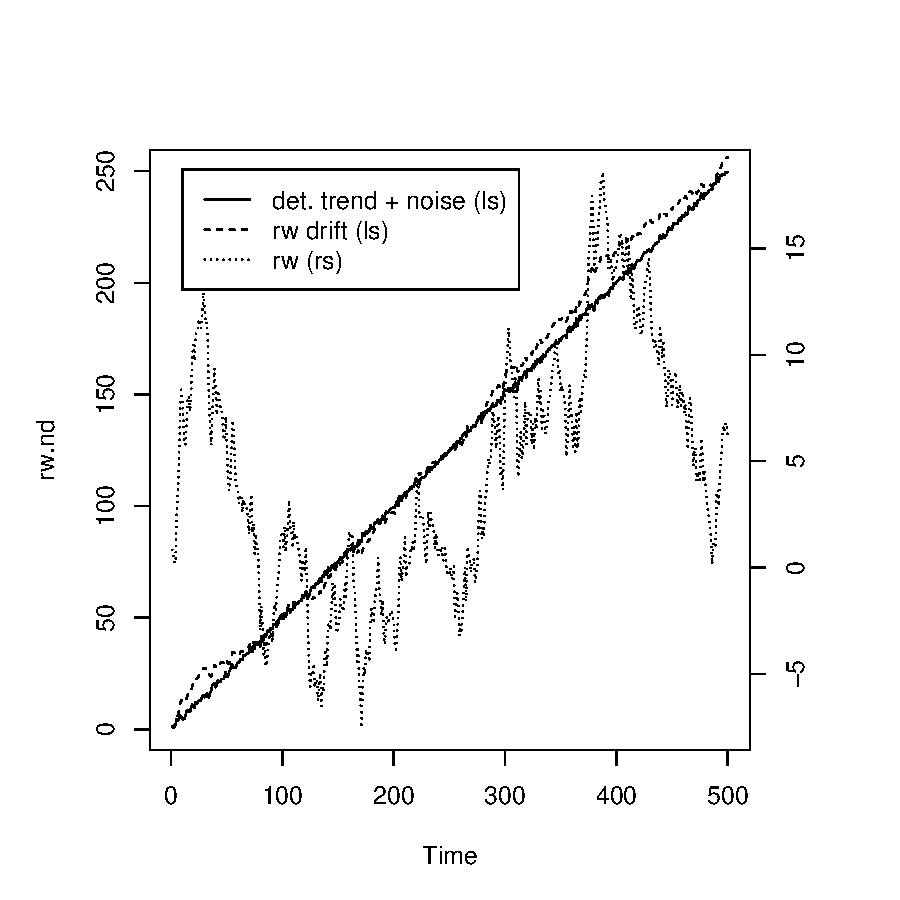
\includegraphics[width=\maxwidth]{figure/plotting} \caption[Three Series]{Three Series\label{fig:plotting}}
\end{figure}


\end{knitrout}

There are also a series of tests that can be used to determine the nature of the time series.  There are three types of statonary series to be identified:  \emph{trend stationary}, \emph{difference stationary} and \emph{difference stationary with drift}.

\subsection{Dickey-Fuller Tests}

Equation \ref{eq:gen} can be used to estimate all three types of series. 
\begin{equation}
\label{eq:gen}
y_t = \beta_1 + \beta_2 t + \rho y_{t-1} +\sum_{j=1}^k \gamma_j \Delta y_i + u_{1t}
\end{equation}
However, rather than testing the unit root as $\rho$ being equal to unity, it is more usual to take $y_{t-1}$ is taken from each side to produce the following adaption of Equation \ref{eq:gen}. 

\begin{equation}
\Delta y_t = \beta_1 + \beta_2 t + \pi y_{t-1} +\sum_{j=1}^k \gamma_j \Delta y_i + u_{1t}
\label{eq:df}
\end{equation}

where $\pi = 1 - \rho$ and therefore if $\pi$ is significantly different from zero, $\rho$ cannot be one and there is no unit root. 

Lags of the dependent variable are used to remove any serial correlation in the residuals. \emph{Information Criteria} and t-statistics can be used to assess the appropriate number of lags

Using the usca package and the ur.df function on UK real consumer spending data (lc). Set up the data as a timeseries.   

\begin{knitrout}
\definecolor{shadecolor}{rgb}{0.969, 0.969, 0.969}\color{fgcolor}\begin{kframe}
\begin{alltt}
\hlfunctioncall{library}(urca)
\hlfunctioncall{library}(xtable)
\hlfunctioncall{data}(Raotbl3)
lc <- \hlfunctioncall{ts}(Raotbl3$lc, start = \hlfunctioncall{c}(1966, 4), end = \hlfunctioncall{c}(1991, 2), frequency = 4)
\end{alltt}
\end{kframe}
\end{knitrout}

\begin{knitrout}
\definecolor{shadecolor}{rgb}{0.969, 0.969, 0.969}\color{fgcolor}\begin{figure}[h]

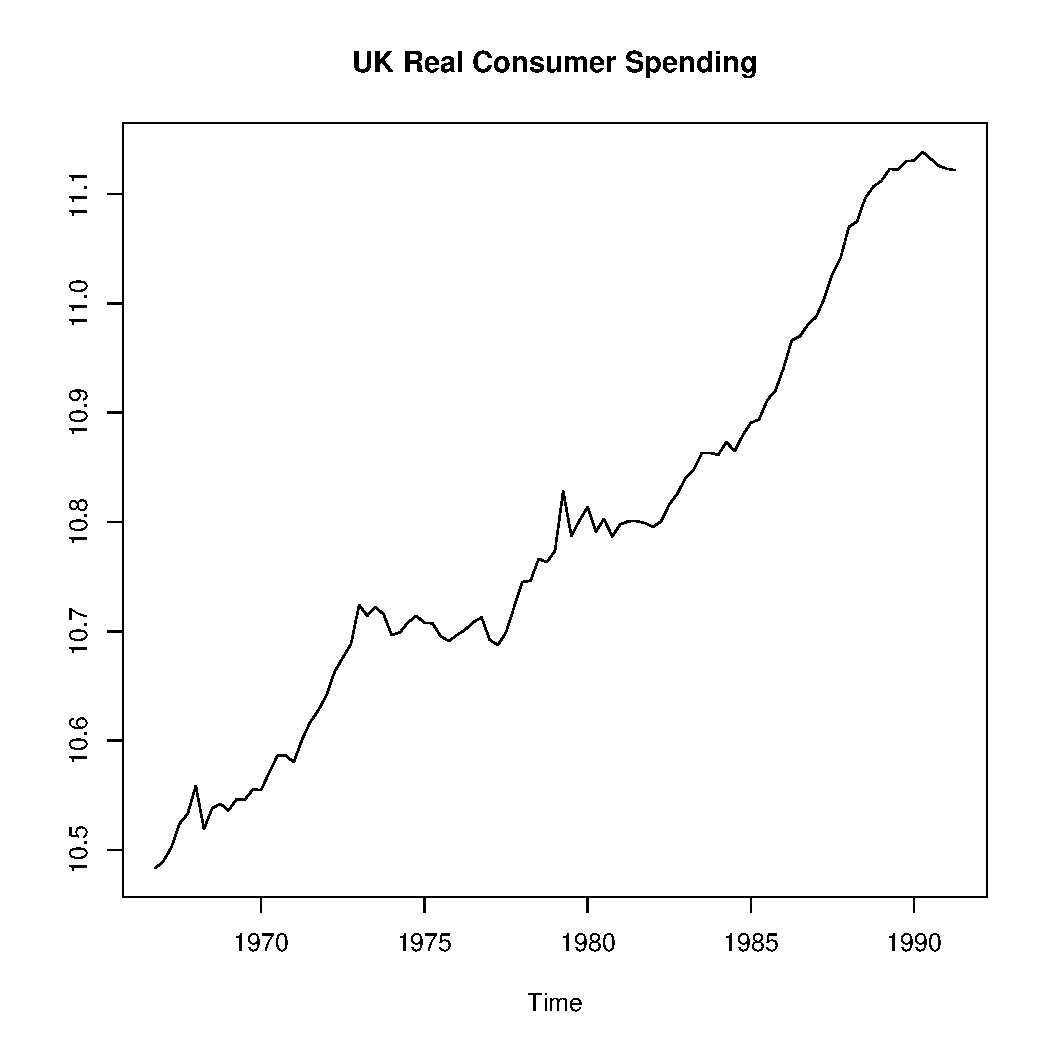
\includegraphics[width=\maxwidth]{figure/plotlc} \caption[Log UK Consumer Spending]{Log UK Consumer Spending\label{fig:plotlc}}
\end{figure}


\end{knitrout}

Conduct the Augmented Dickey-Fuller test on (lc.ct) trend and (lc.co) drift using three lags. 
\begin{knitrout}
\definecolor{shadecolor}{rgb}{0.969, 0.969, 0.969}\color{fgcolor}\begin{kframe}
\begin{alltt}
lc.ct <- \hlfunctioncall{ur.df}(lc, lags = 3, type = \hlstring{"trend"})
lc.co <- \hlfunctioncall{ur.df}(lc, lags = 3, type = \hlstring{"drift"})
\end{alltt}
\end{kframe}
\end{knitrout}

The three different equations are tested by 'trend', 'drift' or 'none' and there are two tests that take place. 

The first $(\tau_3)$ tests whether $\pi$ is equal to zero.  The test is the usual t-value on the lagged dependent variable. This can seen in the summary() function or the SlotName "teststat".  The critical values for the test statistics are in the slotName "cval".  The following code extracts the relevant values and puts them into a table. 
\begin{kframe}
\begin{alltt}
a <- \hlfunctioncall{cbind}(\hlfunctioncall{t}(lc.ct@teststat), lc.ct@cval)
\hlfunctioncall{print}(\hlfunctioncall{xtable}(a, digits = 2, caption = \hlstring{"DW and F-tests"}))
\end{alltt}
\end{kframe}% latex table generated in R 2.15.2 by xtable 1.7-0 package
% Sun Jun 09 16:25:47 2013
\begin{table}[ht]
\begin{center}
\begin{tabular}{rrrrr}
  \hline
 & statistic & 1pct & 5pct & 10pct \\ 
  \hline
tau3 & -2.24 & -4.04 & -3.45 & -3.15 \\ 
  phi2 & 3.74 & 6.50 & 4.88 & 4.16 \\ 
  phi3 & 2.60 & 8.73 & 6.49 & 5.47 \\ 
   \hline
\end{tabular}
\caption{DW and F-tests}
\end{center}
\end{table}



The $\tau_3$ test statistic is the test of the null hypothesis that the coefficient on the difference of the lagged dependent variable is equal to zero and that there is a \emph{unit root} as $\rho$ is equal to one.  


The critical value for a sample size of 100 comes from \citep{Fuller1976}. 

An F-test of the null hypothesis that the coefficients on the lagged change in the dependend variable and the coefficient on the time trend are jointly equal to zero is also supplied $(\phi_3)$.  The critical values come from Table VI \citep{DF1981} testing the null $(\alpha, \beta, \rho) = (\alpha, 0, 1)$.  It seems that unit root and lack of time trend cannot be rejected. A joint test of the null that the coefficients on the drift, time trend and lagged difference of the dependent variable is suppoed in $(\phi_2)$.  The critical values come from Table V \citep{DF1981} testing the null $(\alpha, \beta, \rho) = (0, 0, 1)$.

As the consumption series does not appear to be trend stationary, a test without the trend can be carried out.  This is equivalent to setting $\beta_2$ in Equation \ref{eq:gen} to zero. lc.co is the test of the series with drift.  
\begin{kframe}
\begin{alltt}
a <- \hlfunctioncall{cbind}(\hlfunctioncall{t}(lc.co@teststat), lc.co@cval)
\hlfunctioncall{print}(\hlfunctioncall{xtable}(a, digits = 2, caption = \hlstring{"DW and F-tests 2"}))
\end{alltt}
\end{kframe}% latex table generated in R 2.15.2 by xtable 1.7-0 package
% Sun Jun 09 16:25:47 2013
\begin{table}[ht]
\begin{center}
\begin{tabular}{rrrrr}
  \hline
 & statistic & 1pct & 5pct & 10pct \\ 
  \hline
tau2 & -0.09 & -3.51 & -2.89 & -2.58 \\ 
  phi1 & 2.88 & 6.70 & 4.71 & 3.86 \\ 
   \hline
\end{tabular}
\caption{DW and F-tests 2}
\end{center}
\end{table}


The critical value of 2.88 $(\phi_1)$ is a test of the null that the coefficients on the drift and lagged difference of the dependend variable are jointly equal to zero.  This cannot be rejected.  Therefore, it seems that the log of UK consumer spending is a random walk.  

To complete the picture, the change in consumer spending is tested to maker sure that the series are I(1) rather than I(2). First create the difference series lc2.ct.  
\begin{knitrout}
\definecolor{shadecolor}{rgb}{0.969, 0.969, 0.969}\color{fgcolor}\begin{kframe}
\begin{alltt}
lc2 <- \hlfunctioncall{diff}(lc)
lc2.ct <- \hlfunctioncall{ur.df}(lc2, type = \hlstring{"trend"}, lags = 3)
\end{alltt}
\end{kframe}
\end{knitrout}


\begin{kframe}
\begin{alltt}
a <- \hlfunctioncall{cbind}(\hlfunctioncall{t}(lc2.ct@teststat), lc2.ct@cval)
\hlfunctioncall{print}(\hlfunctioncall{xtable}(a, digits = 2, caption = \hlstring{"DW and F-tests 3"}))
\end{alltt}
\end{kframe}% latex table generated in R 2.15.2 by xtable 1.7-0 package
% Sun Jun 09 16:25:47 2013
\begin{table}[ht]
\begin{center}
\begin{tabular}{rrrrr}
  \hline
 & statistic & 1pct & 5pct & 10pct \\ 
  \hline
tau3 & -4.39 & -4.04 & -3.45 & -3.15 \\ 
  phi2 & 6.45 & 6.50 & 4.88 & 4.16 \\ 
  phi3 & 9.62 & 8.73 & 6.49 & 5.47 \\ 
   \hline
\end{tabular}
\caption{DW and F-tests 3}
\end{center}
\end{table}


This shows that the null of a unit root can be rejected and indicates that the UK consumer spending data are difference stationary.  

\subsection{KPSS}
There are a number of other tests of a unit root in the Bernhard Pfaff text (pages 94 to 102).  These include the \emph{Phillips-Peron}, \emph{Elliot-Rothenberg-Stock} and \emph{Schmidt-Phillips} tests which are implemented by ur.pp, ur.ers and ur.sp respectively in the urca package.  However, these all test the null of a unit root.  The \emph{Kwiatkowski-Phillips-Schmidt-Shin Test} \citep{KPSS} tests the null stationarity.  This is a much more powerful test and can be used in conjunction with the more conventional tests.  If the other tests suggest a unit root but the KPSS rejects a unit root, it is probably best to consider the data as stationary. 

The KPSS test is of the form
\begin{equation}
\label{eq:KPSS}
y_t = \zeta t + r_t + \varepsilon_t
\end{equation}

\begin{equation}
r_t = r_{t-1} + u_t
\end{equation}

The test statistic is calculated by running the regression of $y$ on a constant and trend as in Equation \ref{eq:KPSS} or on just a constant as in equation \ref{eq:KPSS} with $\zeta$ equal to zero.    

\begin{equation}
LM = \frac{\sum_{i = 1}^T S_t^2}{\hat{\sigma_t^2}}
\end{equation}
where 
\begin{equation}
S_t = \sum_{i = 1}^t \hat{\varepsilon} , t = 1, 2,...T
\end{equation}
and the estimate of the error variance
\begin{equation}
\hat{\sigma_{\varepsilon}}^2 = s^2 (l) = T^{-1} \sum_{t=1}^T \varepsilon_t^2 +2T - 1 \sum_{s=1}^l 1-\frac{s}{l+1} \sum_{t=s+1}^T \hat{\varepsilon} \hat{\varepsilon}_{t-1}
\end{equation}

Using the urca package and the data for US interest rates and nominal wages, the KPSS test is either on level statonary (type = $\mu$) or trend stationary (type = $\tau$) and the lags for the error term are either specified (as below) or set to "short" $\root 4 \of {4 \times (n/100)}$ or "long" $\root 4 \of {12 \times (n/100)}$.
\begin{knitrout}
\definecolor{shadecolor}{rgb}{0.969, 0.969, 0.969}\color{fgcolor}\begin{kframe}
\begin{alltt}
\hlfunctioncall{data}(nporg)
ir <- \hlfunctioncall{na.omit}(nporg[, \hlstring{"bnd"}])
wg <- \hlfunctioncall{log}(\hlfunctioncall{na.omit}(nporg[, \hlstring{"wg.n"}]))
\end{alltt}
\end{kframe}
\end{knitrout}

Plot the data
\begin{knitrout}
\definecolor{shadecolor}{rgb}{0.969, 0.969, 0.969}\color{fgcolor}\begin{kframe}
\begin{alltt}
\hlfunctioncall{par}(mfrow = \hlfunctioncall{c}(2, 1))
\hlfunctioncall{plot.ts}(ir, main = \hlstring{"US interest rates"})
\hlfunctioncall{plot.ts}(wg, main = \hlstring{"US nominal wages"})
\end{alltt}
\end{kframe}\begin{figure}[h]

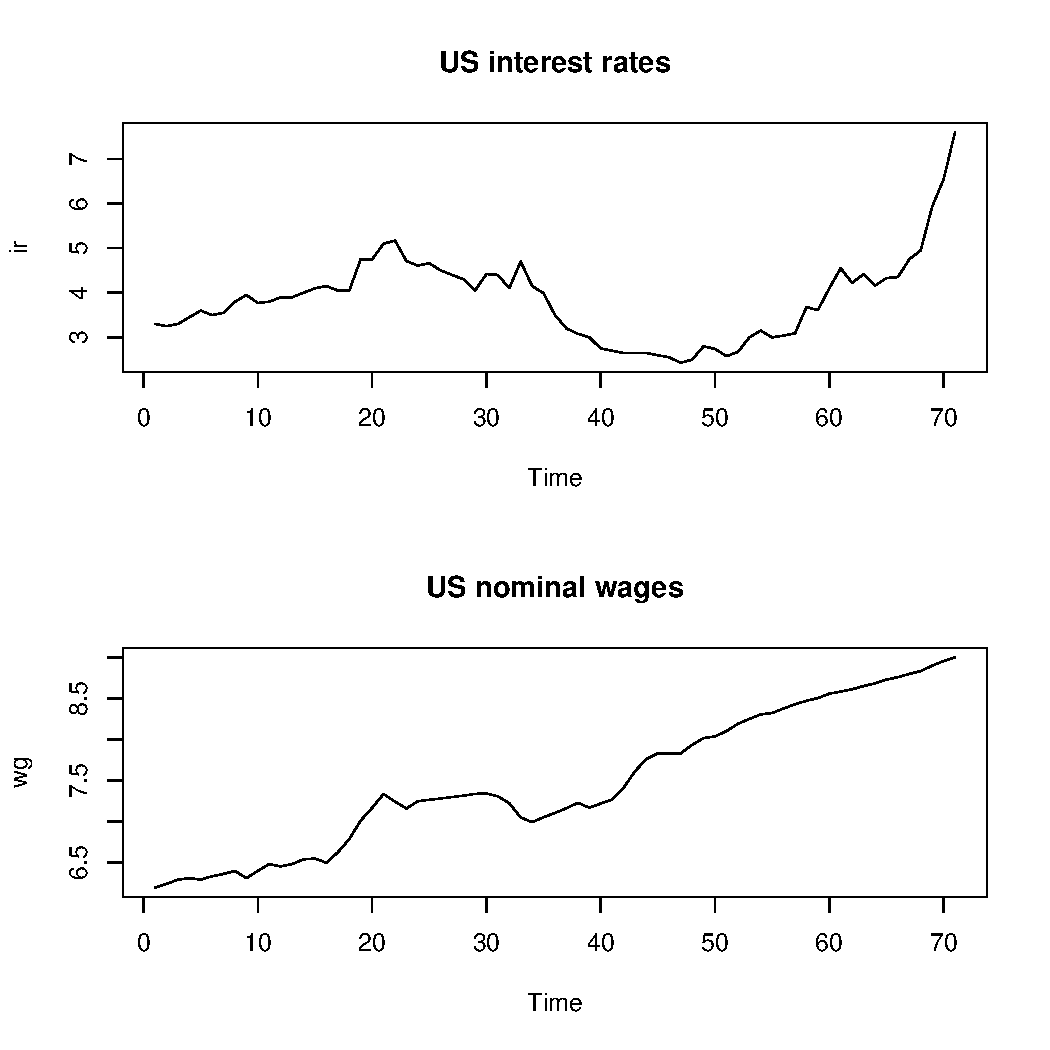
\includegraphics[width=\maxwidth]{figure/plot-kpss} \caption[US interest rate and wage data]{US interest rate and wage data\label{fig:plot-kpss}}
\end{figure}


\end{knitrout}


\begin{knitrout}
\definecolor{shadecolor}{rgb}{0.969, 0.969, 0.969}\color{fgcolor}\begin{kframe}
\begin{alltt}
ir.kpss <- \hlfunctioncall{ur.kpss}(ir, type = \hlstring{"mu"}, use.lag = 8)
wg.kpss <- \hlfunctioncall{ur.kpss}(wg, type = \hlstring{"tau"}, use.lag = 8)
\end{alltt}
\end{kframe}
\end{knitrout}

And the appropriate data can be extracted and placed into a table using the following. 
\begin{kframe}
\begin{alltt}
a <- \hlfunctioncall{cbind}(ir.kpss@teststat, ir.kpss@cval)
b <- \hlfunctioncall{cbind}(wg.kpss@teststat, wg.kpss@cval)
ab <- \hlfunctioncall{rbind}(a, b)
\hlfunctioncall{colnames}(ab) <- \hlfunctioncall{c}(\hlstring{"CV"}, \hlstring{"10pct"}, \hlstring{"5pct"}, \hlstring{"2.5pct"}, \hlstring{"1.0pct"})
\hlfunctioncall{rownames}(ab) <- \hlfunctioncall{c}(\hlstring{"ir"}, \hlstring{"wg"})
\hlfunctioncall{print}(\hlfunctioncall{xtable}(ab, digits = 2, caption = \hlstring{"KPSS and critical values"}))
\end{alltt}
\end{kframe}% latex table generated in R 2.15.2 by xtable 1.7-0 package
% Sun Jun 09 16:25:47 2013
\begin{table}[ht]
\begin{center}
\begin{tabular}{rrrrrr}
  \hline
 & CV & 10pct & 5pct & 2.5pct & 1.0pct \\ 
  \hline
ir & 0.13 & 0.35 & 0.46 & 0.57 & 0.74 \\ 
  wg & 0.10 & 0.12 & 0.15 & 0.18 & 0.22 \\ 
   \hline
\end{tabular}
\caption{KPSS and critical values}
\end{center}
\end{table}


This shows that the null hypothesis of level stationarity for the interest rate series and trend stationarity for the wage series cannnot be rejected.  


\section{Cointegration}
This is the overview of conintegration and the methods use to analyse conintegrated relationships. Non-stationary data may exhibit \emph{spurious regression}.  If two norman random variables are created (e1 and e2) and two series (y1 and y2) have a trend plus a random shock. 
\begin{knitrout}
\definecolor{shadecolor}{rgb}{0.969, 0.969, 0.969}\color{fgcolor}\begin{kframe}
\begin{alltt}
\hlfunctioncall{library}(lmtest)
\hlfunctioncall{library}(xtable)
\hlfunctioncall{set.seed}(123456)
e1 <- \hlfunctioncall{rnorm}(500)
e2 <- \hlfunctioncall{rnorm}(500)
trd <- 1:500
y1 <- 0.8 * trd + \hlfunctioncall{cumsum}(e1)
y2 <- 0.6 * trd + \hlfunctioncall{cumsum}(e2)
\end{alltt}
\end{kframe}
\end{knitrout}

Now plot the two series
\begin{knitrout}
\definecolor{shadecolor}{rgb}{0.969, 0.969, 0.969}\color{fgcolor}\begin{kframe}
\begin{alltt}
\hlfunctioncall{plot}(y1, type = \hlstring{"l"}, main = \hlstring{"Plot of y1 and y2"}, col = \hlstring{"red"}, ylab = \hlstring{"y1, y2"})
\hlfunctioncall{lines}(y2, col = \hlstring{"blue"})
\end{alltt}
\end{kframe}
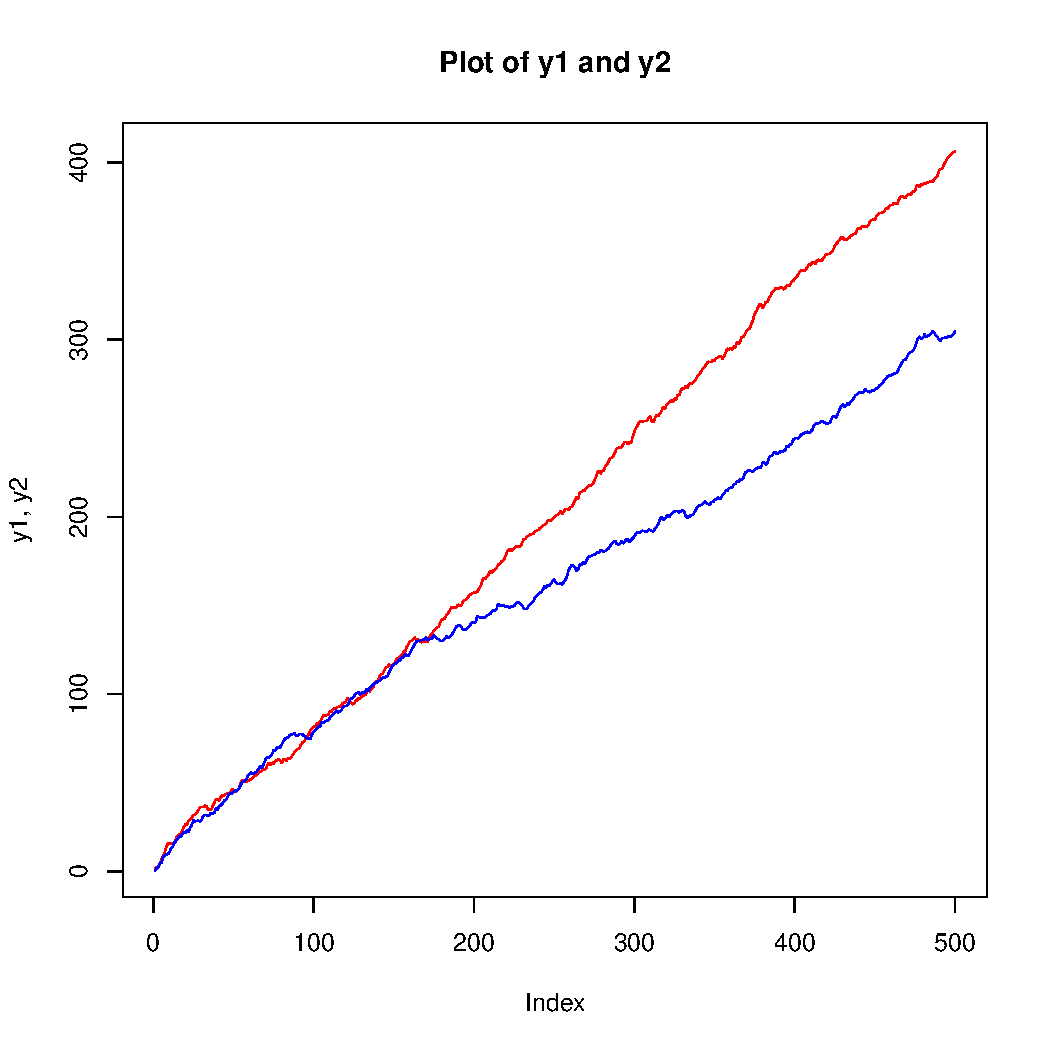
\includegraphics[width=\maxwidth]{figure/plot} 

\end{knitrout}

Run a regression of $y1$ on $y2$ and it appears that there is a strong relationship.  
\begin{kframe}
\begin{alltt}
sr.reg <- \hlfunctioncall{lm}(y1 ~ y2)
\hlfunctioncall{print}(\hlfunctioncall{xtable}(sr.reg))
\end{alltt}
\end{kframe}% latex table generated in R 2.15.2 by xtable 1.7-0 package
% Sun Jun 09 16:25:48 2013
\begin{table}[ht]
\begin{center}
\begin{tabular}{rrrrr}
  \hline
 & Estimate & Std. Error & t value & Pr($>$$|$t$|$) \\ 
  \hline
(Intercept) & -29.3270 & 1.3672 & -21.45 & 0.0000 \\ 
  y2 & 1.4408 & 0.0075 & 191.62 & 0.0000 \\ 
   \hline
\end{tabular}
\end{center}
\end{table}


However, the Durbin-Watson statistics shows there is a large amount of auto-correlation in the residuals.  
\begin{knitrout}
\definecolor{shadecolor}{rgb}{0.969, 0.969, 0.969}\color{fgcolor}\begin{kframe}
\begin{alltt}
sr.dw <- \hlfunctioncall{dwtest}(sr.reg)$statistic
sr.dw
\end{alltt}
\begin{verbatim}
##      DW 
## 0.01715
\end{verbatim}
\end{kframe}
\end{knitrout}

The statistic will be around 2 if there is no autocorrelation. 
\newpage
\bibliography{myref}
\bibliographystyle{agsm}


\end{document}
